% ============================================================
% ConsistXApp -- final manuscript
% Target journal: Annals of Telecommunications (sn-jnl.cls)
% ============================================================

\documentclass[pdflatex,sn-mathphys-num,iicol,oneside]{sn-jnl}

\usepackage{amsmath}
\usepackage{amssymb}
\usepackage{bm}
\usepackage{booktabs}
\usepackage{array}
\usepackage{tikz}
\usepackage{url}
\usepackage{graphicx}
\usepackage{float}

\floatstyle{ruled}
\newfloat{algorithm}{t}{loa}
\floatname{algorithm}{Algorithm}
\newcommand{\algin}[1]{\textbf{Input:} #1\par}
\newcommand{\algout}[1]{\textbf{Output:} #1\par\vspace{2pt}\hrule\vspace{3pt}}
\newenvironment{algsteps}%
  {\begin{list}{\arabic{algstepc}:}%
     {\usecounter{algstepc}\setlength{\leftmargin}{1.6em}%
      \setlength{\itemsep}{1pt}\setlength{\parsep}{0pt}}}%
  {\end{list}}
\newcounter{algstepc}

\usetikzlibrary{arrows.meta,positioning,fit,shapes.geometric}

\newcommand{\method}{\textsc{ConsistXApp}}
\newcommand{\gac}{\textsc{GAC}}
\newcommand{\cpsat}{\textsc{CP-SAT}}

\newtheorem{proposition}{Proposition}
\newtheorem{definition}{Definition}
\newtheorem{remark}{Remark}

\raggedbottom

\begin{document}

\title[Consistency-Guided xApp Coordination]{
Consistency-Guided xApp Coordination in the Near-RT RIC:
Incremental Propagation, Explanation-Guided Exact Repair,
and Independently Verified Decisions
}

\author*[1]{\fnm{Lillia} \sur{Ouali}}
\email{lillia.ouali@univ-bejaia.dz}

\author[2]{\fnm{Madani} \sur{Bezoui}}
\email{mbezoui@cesi.fr}

\author[1]{\fnm{Kamal} \sur{Amroun}}
\email{kamal.amroun@univ-bejaia.dz}

\author[3]{\fnm{Ahcene} \sur{Bounceur}}
\email{abounceur@sharjah.ac.ae}

\affil*[1]{
    \orgdiv{Department of Computer Science},
    \orgname{University of Bejaia},
    \orgaddress{\city{Bejaia}, \country{Algeria}}
}

\affil[2]{
    \orgdiv{LINEACT},
    \orgname{CESI},
    \orgaddress{\city{Nancy}, \country{France}}
}

\affil[3]{
    \orgname{University of Sharjah},
    \orgaddress{\city{Sharjah}, \country{United Arab Emirates}}
}

\abstract{
Independently developed xApps issue concurrent control requests
through the near-real-time RAN Intelligent Controller (RIC) of an
Open RAN, and these requests may be mutually incompatible or jointly
violate service-level agreements. We model multi-xApp arbitration as
a dynamic finite-domain constraint optimization problem and propose
\method, a coordination pipeline that maintains generalized arc
consistency incrementally across decision epochs, repairs invalid
candidate decisions through an exact local subproblem whose scope is
grown by propagation explanations and solver conflict cores, and
forwards an action only after an independent verifier has checked
every registered hard constraint. The verifier is itself validated by
exhaustive enumeration against an independent oracle, a second
implementation sharing no code, property-based testing, and
oracle-labelled input-mutation testing, with zero divergence across
680{,}450 checks. On five O-RAN conflict scenarios, \method\ attains
100\% verified feasibility with a 1.8~ms median latency, faster than
complete \cpsat\ (2.8~ms, paired Wilcoxon $p<10^{-33}$), and every
repair carries an auditable certificate replayable against the
registered model. On the 248 repairs triggered by the operational
pipeline, expanding repair cores succeed where fixed cores fail on
8.5\% of cases (exact McNemar $p<10^{-5}$) while remaining
approximately half the size of full-scope solving. The decisive advantage is amortized: when
2\% of the conflict relations change between epochs, repairing the
previous verified decision costs a median of 0.05--4.9~ms per epoch
for 100--1{,}000 variables, against 2.8--25.6~ms for re-solving from
scratch with or without solution hints, and the advantage holds in
every one of ten paired episodes per size, tail latencies, however,
reach re-solve parity at the 95th percentile and cross over beyond
it. We report the boundaries of the approach with equal weight:
cold-start coordination of isolated instances offers no advantage
over a modern solver, local repair pays a quantified price in
objective quality relative to exact optimization (10.8 points of
kept-request rate on average), and a continuous-relaxation stage that
we evaluated degrades both latency and feasibility and is excluded
from the pipeline.
}

\keywords{
O-RAN, xApp conflict management, dynamic constraint satisfaction,
generalized arc consistency, explanation-based repair,
constraint programming, near-real-time RIC
}

\maketitle

% ============================================================
\section{Introduction}
\label{sec:introduction}
% ============================================================

The Open Radio Access Network (O-RAN) architecture disaggregates the
radio access network and exposes its control through programmable
components. Its near-real-time RAN Intelligent Controller (RIC) hosts
xApps - third-party applications that subscribe to measurements and
issue control requests over the E2 interface within control loops of
tens of milliseconds to one second \cite{polese2023oran}. Because
xApps are developed independently, often by different vendors, they
may simultaneously write the same parameter, steer different
parameters toward incompatible operating points, or jointly violate a
service-level agreement (SLA). The O-RAN Alliance therefore assigns a
conflict-mitigation function to the near-real-time RIC
\cite{oran2024conflict}, and a growing literature classifies xApp
conflicts as direct, indirect, or implicit and proposes detection and
resolution mechanisms \cite{adamczyk2023conflict,wadud2024qacm}.

Most existing mechanisms answer the question of \emph{what} a
candidate action will do to the network, through profiling, digital
twins, learning, or bargaining. This paper addresses the complementary
question that arises once candidate actions and conflict relations
have been registered: how should a controller reason over finite
action domains, under a near-real-time budget, so that only decisions
satisfying every registered hard constraint reach the network - and so
that each intervention can be audited afterwards?

We answer with \method, a coordination pipeline built from three
mechanisms of constraint programming that, to our knowledge, have not
been combined for O-RAN control. First, an \emph{incremental
generalized arc-consistency} (GAC) stage removes candidate actions
that have no support in any incident hard relation, reusing
propagation state across decision epochs and restoring values soundly
when a relation is relaxed. Second, when a decoded candidate violates
some relations, an \emph{explanation-guided exact repair} solves a
small induced subproblem: the violated constraints seed a variable
core, the remaining variables are fixed to their decoded values, and
the core grows only as directed by propagation explanations or by the
solver's own infeasibility cores, escalating to the full model only if
needed. Third, an \emph{independent verifier}, validated against an
exhaustive oracle and a second implementation, gates every forwarded
action. The pipeline is deliberately conservative: it never trusts its
own optimizer.

A modern constraint solver is a demanding yardstick for such a
design. OR-Tools \cpsat\ solves each of our scenario instances from
scratch in under 3~ms, so no coordination layer can justify itself on
isolated instances of that size, we report this honestly rather than
hide it. The case for \method\ is \emph{amortized}. Near-real-time
coordination is a sequence of closely related problems: between two
epochs, only a fraction of the xApps, domains, and context-dependent
relations changes. Re-solving from scratch pays the full model cost at
every epoch - and, as our experiments show, warm-starting the solver
with the previous solution does not reduce that cost, whose measured
components (model construction plus full-model search) both scale with
the model rather than with the change. Repairing the previous verified
decision instead pays a cost proportional to the number of violated
relations. At one thousand variables with 2\% of relations changing
per epoch, verified local repair is five times faster in the median
than either evaluated re-solve strategy, and the gap widens with model
size.

The contributions of this paper are as follows. We formulate
multi-xApp coordination as a dynamic finite-domain constraint
optimization problem with context-dependent hard relations and a
temporal-stability objective. We design an incremental GAC layer with
sound value restoration after relaxations, prove that its filtering
preserves every globally feasible assignment, and show by a symmetric
counterexample why filtering alone cannot guarantee valid decoding.
We introduce explanation-guided exact repair with monotone core
expansion and conditional completeness, on the repairs triggered by
the operational pipeline, expanding cores succeed significantly more
often than fixed cores and remain approximately half the size of
full-scope solving at a lower cost. We validate the independent verifier through four
gates - exhaustive oracle, second implementation, property-based
testing, oracle-labelled input mutation - which, to our knowledge,
have not previously been reported for O-RAN conflict management.
Finally, we characterize the operational regime of the architecture
with paired, multiplicity-corrected statistics at the episode level:
no cold-start advantage at up to 1{,}000 variables, a growing
amortized median advantage in sequential operation with honestly
reported tail behaviour, a quantified objective-quality gap relative
to exact optimization, and a negative result for a
continuous-relaxation stage that we evaluated and excluded.

Section~\ref{sec:background} reviews related work.
Section~\ref{sec:model} defines the coordination model.
Section~\ref{sec:method} presents \method\ and
Section~\ref{sec:analysis} its properties.
Sections~\ref{sec:experiments} and~\ref{sec:results} describe the
experimental setup and results. Section~\ref{sec:limitations}
discusses limitations and Section~\ref{sec:conclusion} concludes.

% ============================================================
\section{Background and Related Work}
\label{sec:background}
% ============================================================

The near-real-time RIC supports control loops between tens of
milliseconds and one second, xApps subscribe to key performance
measurements (KPMs), process network context, and issue E2 control
requests \cite{polese2023oran}. Experimental frameworks such as
ColO-RAN, OpenRAN Gym, and FlexRIC support the development and
closed-loop evaluation of such controllers
\cite{polese2022coloran,bonati2023openrangym,schmidt2021flexric}.
Three conflict classes are commonly distinguished
\cite{adamczyk2023conflict}. A \emph{direct} conflict arises when two
xApps request incompatible values of the same parameter, for example a
coverage xApp raising transmission power that an energy-saving xApp is
lowering. An \emph{indirect} conflict arises when different controlled
parameters influence a common KPM, as when cell-individual offsets and
handover thresholds jointly determine user association. An
\emph{implicit} conflict couples distinct parameters and KPMs through
network dynamics, as when sleeping a cell degrades mobility
robustness. Direct conflicts are checkable syntactically, indirect and
implicit conflicts require a registered parameter--KPM dependency
model, a profile, or a conservative operator rule.

Proposed management mechanisms span a conflict-mitigation framework
embedded in the RIC \cite{adamczyk2023conflict}, QoS-aware
optimization that maximizes the number of xApps whose requirements are
met \cite{wadud2024qacm,annals2024}, cooperative bargaining over
conflicting parameters \cite{wadud2023game}, pre-deployment profiling
with statistical models and hierarchical graphs
\cite{prever2025pacifista}, digital-twin-based impact evaluation
\cite{giannopoulos2025comix}, and rule-based mitigation in
mobility-versus-energy case studies \cite{wadud2025mobility}. Closest
to our auditability goal, XAI4C applies explainable-AI techniques to
conflict detection and mitigation \cite{varshney2025xai4c}, its
explanations are post-hoc attributions of a learned detector, whereas
the explanations produced here are logical premises replayable against
the registered constraint model and checkable by an independent
program.

On the constraint-programming side, propagation removes domain values
that cannot participate in any locally supported tuple, for non-binary
relations this is generalized arc consistency, efficiently enforceable
for positive table constraints by simple tabular reduction and its
successors \cite{yap2020gac,lecoutre2011str2}. Local consistency is
not a decision procedure - a GAC network may admit no solution - but
it detects some contradictions without search and shrinks the space
handed to an exact solver. Dynamic constraint satisfaction studies
sequences of related problems and incremental consistency maintenance
\cite{bessiere1991dynamic}, and explanations that justify value
removals or contradictions support diagnosis and repair
\cite{gupta2021explanations}. Modern solvers such as OR-Tools \cpsat\
combine presolve, propagation, clause learning, and optimization
\cite{perron2023cpsat,ortools}, which makes them both a component of
our repair stage and the baseline any coordination layer must face.
The contribution of this work is the integration of incremental
propagation, explanation-guided local repair, and independently
validated verification into a budget-aware xApp coordination
loop, together with an evaluation that identifies the regime - 
sequential, not cold-start - in which the integration pays.

% ============================================================
\section{System Model}
\label{sec:model}
% ============================================================

\subsection{Epochs, actions, and context-dependent relations}

The near-real-time RIC operates over decision epochs $t=1,\ldots,T$.
At epoch $t$, each active xApp action variable $i\in\mathcal{A}_t$ has
a finite base domain $D_i^t=\{a_{i,1}^t,\ldots,a_{i,d_i}^t\}$ whose
values encode concrete controls: accepting or rejecting a request,
selecting a target cell or an execution slot, choosing a discrete
power level, a handover offset, or a resource-allocation profile, or
executing a registered safe no-operation. The discrete variable
$x_i^t\in D_i^t$ is the coordinated action selected for variable $i$,
the time index is omitted when a single epoch is considered.

A constraint $c\in\mathcal{C}_t$ has scope $S_c\subseteq\mathcal{A}_t$
and an allowed relation
\begin{equation}
R_c(\bm{s}_t)\subseteq\prod_{i\in S_c}D_i^t,
\end{equation}
where $\bm{s}_t$ is the observed and registered network context. An
assignment $\bm{x}^t$ satisfies $c$ if
$\bm{x}_{S_c}^t\in R_c(\bm{s}_t)$. Relations may be binary or
higher-order and are generated from operator policies, parameter
ownership, SLA and QoS thresholds, validated xApp profiles, a
calibrated simulator or digital twin, or conservative safety rules.
Hard constraints must hold before a decision executes, soft
constraints only contribute to utility. The hard model at epoch $t$ is
$\mathcal{M}_t=(\mathcal{A}_t,\bm{D}_t,\mathcal{C}_t,\bm{s}_t)$.

Between epochs, xApps activate or deactivate, candidate actions and
constraints appear or disappear, relations tighten or relax, and SLA
thresholds move. The modified variables and constraints form the
change set $\Delta_t$. Restrictive and relaxing updates must be
distinguished: after a restriction, previous support information
remains reusable, whereas after a relaxation a previously removed
value may have regained support and must be restored from its base
domain before propagation is re-established
(Proposition~\ref{prop:restoration}).

\subsection{Objective}

Let $u_i(a_i,\bm{s}_t)$ be the utility of selecting action $a_i$ for
variable $i$, weighted by $\omega_i\geq0$, and let $v_q\ge 0$ be
soft-violation penalties with weights $\lambda_q$. The static utility
is
\begin{equation}
U(\bm{x},\bm{s}_t)=\sum_{i\in\mathcal{A}_t}\omega_i u_i(x_i,\bm{s}_t)
-\sum_{q\in\mathcal{Q}_t}\lambda_q v_q(\bm{x},\bm{s}_t).
\label{eq:static-utility}
\end{equation}
With $\bm{x}^{t-1}$ the previous verified decision and
$\kappa_i\geq 0$ reconfiguration costs, the weighted action churn is
\begin{equation}
H(\bm{x}^{t},\bm{x}^{t-1})=
\sum_{i\in\mathcal{A}_t\cap\mathcal{A}_{t-1}}
\kappa_i\,\mathbf{1}\!\left[x_i^t\neq x_i^{t-1}\right],
\label{eq:churn}
\end{equation}
and the coordination problem at epoch $t$ is
\begin{align}
\max_{\bm{x}^{t}}\quad&
U(\bm{x}^{t},\bm{s}_t)-\mu\,H(\bm{x}^{t},\bm{x}^{t-1})
\label{eq:problem-objective}\\
\text{s.t.}\quad&
x_i^t\in D_i^t, \quad i\in\mathcal{A}_t,
\nonumber\\
&\bm{x}_{S_c}^t\in R_c(\bm{s}_t),\quad c\in\mathcal{C}_{t,\mathrm{hard}},
\label{eq:problem-hard}
\end{align}
where $\mu\geq0$ trades instantaneous utility against temporal
stability. Dwell-time and cooldown rules are hard relations when their
violation is not permitted.

\subsection{Worked example}
\label{sec:worked-example}

Consider one cell with a coverage xApp controlling power
$x_1\in\{\text{low},\text{med},\text{high}\}$, an energy-saving xApp
controlling the cell state $x_2\in\{\text{sleep},\text{on}\}$, and two
SLAs (minimum edge throughput, maximum handover-failure rate). The
registered relation
$R_{12}=\{(\text{med},\text{on}),(\text{high},\text{on}),
(\text{low},\text{sleep})\}$
forbids raising coverage from a sleeping cell and forbids low power on
an active cell. Suppose the xApps \emph{request} $x_1=\text{high}$ and
$x_2=\text{sleep}$, requests are soft preferences that enter decoding
through utility, while the base domains remain multivalued (a hard
singleton restriction would instead be detected as a wipeout by
propagation). GAC removes nothing: \text{high} is supported by
$(\text{high},\text{on})$ and \text{sleep} by
$(\text{low},\text{sleep})$, yet the jointly decoded request violates
$R_{12}$.
The verifier rejects it, the violated relation seeds the repair core
$\{x_1,x_2\}$, and exact repair returns a verified alternative such as
$(\text{high},\text{on})$ - or $(\text{low},\text{sleep})$ if the
energy SLA dominates. Propagation prunes unsupported actions, repair
resolves incompatible combinations of individually supported actions.
% ============================================================
\section{The \method\ Framework}
\label{sec:method}
% ============================================================

Figure~\ref{fig:architecture} positions \method\ in the near-real-time
RIC control path: candidate xApp actions are filtered by incremental
GAC, decoded, repaired when necessary, and independently verified
before any E2 message is emitted.

\begin{figure*}[t]
\centering
\resizebox{\textwidth}{!}{%
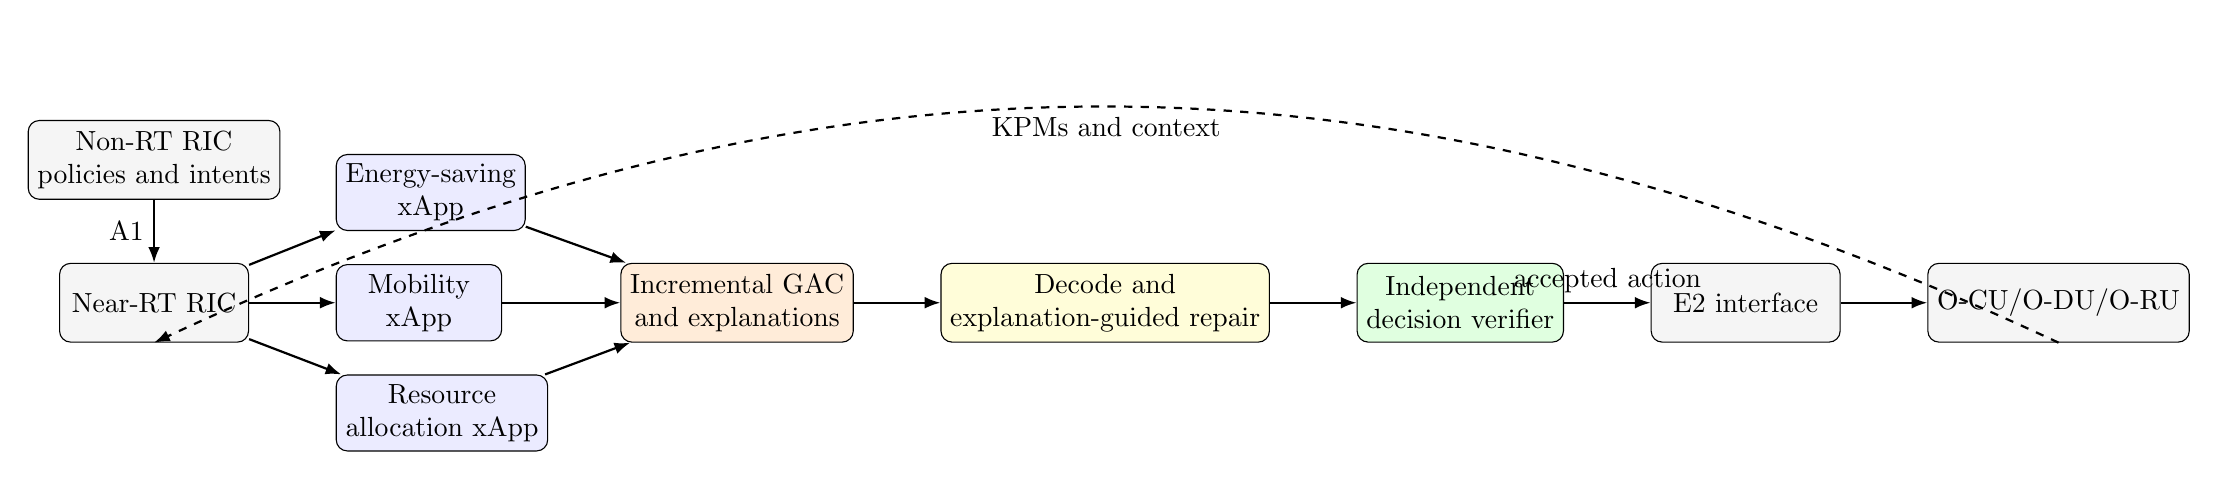
\begin{tikzpicture}[
    node distance=8mm and 11mm,
    block/.style={draw,rounded corners,align=center,
        minimum width=24mm,minimum height=10mm,fill=gray!8},
    app/.style={draw,rounded corners,align=center,
        minimum width=21mm,minimum height=9mm,fill=blue!8},
    prop/.style={draw,rounded corners,align=center,
        minimum width=26mm,minimum height=10mm,fill=orange!15},
    coord/.style={draw,rounded corners,align=center,
        minimum width=27mm,minimum height=10mm,fill=yellow!15},
    verify/.style={draw,rounded corners,align=center,
        minimum width=25mm,minimum height=10mm,fill=green!12},
    arrow/.style={-{Latex[length=2mm]},thick}
]
\node[block] (nonrt) {Non-RT RIC\\policies and intents};
\node[block, below=of nonrt] (near) {Near-RT RIC};
\node[app, right=of near, yshift=14mm] (x1) {Energy-saving\\xApp};
\node[app, right=of near] (x2) {Mobility\\xApp};
\node[app, right=of near, yshift=-14mm] (x3) {Resource\\allocation xApp};
\node[prop, right=15mm of x2] (gac) {Incremental GAC\\and explanations};
\node[coord, right=of gac] (coord) {Decode and\\explanation-guided repair};
\node[verify, right=of coord] (verifier) {Independent\\decision verifier};
\node[block, right=of verifier] (e2) {E2 interface};
\node[block, right=of e2] (ran) {O-CU/O-DU/O-RU};
\draw[arrow] (nonrt) -- node[left]{A1} (near);
\draw[arrow] (near) -- (x1);
\draw[arrow] (near) -- (x2);
\draw[arrow] (near) -- (x3);
\draw[arrow] (x1) -- (gac);
\draw[arrow] (x2) -- (gac);
\draw[arrow] (x3) -- (gac);
\draw[arrow] (gac) -- (coord);
\draw[arrow] (coord) -- (verifier);
\draw[arrow] (verifier) -- node[above]{accepted action} (e2);
\draw[arrow] (e2) -- (ran);
\draw[arrow,dashed] (ran.south) to[bend right=25]
node[below]{KPMs and context} (near.south);
\end{tikzpicture}
}
\caption{\method\ in the near-real-time RIC control path. Incremental
generalized arc consistency filters unsupported actions, propagation
explanations guide exact local repair, and every final action is
independently verified before reaching E2.}
\label{fig:architecture}
\end{figure*}

\subsection{Incremental consistency filtering}
\label{sec:gac}

The propagation stage maintains, next to each base domain $D_i$, a
filtered domain $D_i^{*}\subseteq D_i$, the separation matters because
a later relaxation may restore support for a removed value. The
support set of value $a\in D_i$ in constraint $c$ is
\begin{equation}
\begin{aligned}
\operatorname{Supp}_{c}(i,a;\bm{D})=
\bigl\{\bm{z}\in R_c(\bm{s}_t):\;
&z_i=a \;\land\\[-1pt]
&z_j\in D_j,\;\forall j\in S_c\bigr\},
\end{aligned}
\label{eq:support}
\end{equation}
and a hard network is \emph{generalized arc consistent} when every
value of every variable has a non-empty support in every incident
relation. The revision operator
\begin{equation}
\operatorname{Revise}_{c,i}(\bm{D}):\;
D_i\leftarrow
\{a\in D_i:\operatorname{Supp}_{c}(i,a;\bm{D})\neq\varnothing\}
\label{eq:revise}
\end{equation}
is applied through a propagation queue until a fixed point
$\bm{D}^{*}=\operatorname{GAC}(\bm{D},\mathcal{C}_{\mathrm{hard}},\bm{s}_t)$
is reached. An empty filtered domain (a \emph{wipeout}) proves that no
feasible assignment extends the current domains, the converse does not
hold.

Across epochs, the propagator works incrementally
(Algorithm~\ref{alg:incgac}). The queue is seeded only with the
constraints affected by $\Delta_t$ and those sharing an affected
variable. For a purely restrictive transition, cached supports and
previous deletions are reused as long as their premises remain valid.
For a transition containing a relaxation, the affected connected
component is first restored to its base domains and current allowed
tuples, then consistency is re-established, this restoration rule
prevents stale deletions from being carried unsoundly across a relaxed
context. For explicit positive tables the implementation records the
active tuples, the last known support of each variable--value pair,
the context identifier under which that support was valid, and the
explanation of each removal, these caches accelerate propagation
without changing the fixed-point semantics.

\subsection{Propagation explanations}
\label{sec:explanations}

When value $a$ is removed from $D_i$ by constraint $c$, the propagator
records an explanation
$\mathcal{E}(i,a)\subseteq\mathcal{C}_{\mathrm{hard}}\cup\mathcal{L}$,
where $\mathcal{L}$ collects temporary domain restrictions and
boundary decisions. The explanation contains premises sufficient to
establish that every tuple of $R_c$ assigning $a$ to $x_i$ is
incompatible with the current domains: for each candidate support
tuple, at least one premise states why that tuple is inactive. A
wipeout explanation for variable $i$ is the union
$\mathcal{E}_{\emptyset}(i)=\bigcup_{a}\mathcal{E}(i,a)$ over its
removed base values. Explanations are not required to be
cardinality-minimal, they are required to be logically valid relative
to the registered model, reproducible from the propagation trace,
bound to a context identifier, and accepted by a separately
implemented explanation checker that replays the premises and verifies
that every supporting tuple is disabled.

\subsection{Decoding and explanation-guided exact repair}
\label{sec:repair}

If propagation ends without wipeout, a deterministic decode
$\widehat{x}_i\in D_i^{*}$ selects, per variable, the
maximum-utility (or documented tie-broken) value of the filtered
domain. Local support does not imply joint validity
(Section~\ref{sec:analysis}), so the decoded candidate is tested and,
if it violates hard relations, repaired exactly
(Algorithm~\ref{alg:repair}).

The violated relations
$\mathcal{C}^{0}=\{c:\widehat{\bm{x}}_{S_c}\notin R_c(\bm{s}_t)\}$
seed the variable core
$\mathcal{A}^{0}=\bigcup_{c\in\mathcal{C}^{0}}S_c$. At iteration $r$,
variables outside the core are fixed to their decoded values and
variables inside retain their filtered domains, GAC is enforced on
this induced model and the subproblem is passed to \cpsat. The
expansion order is deterministic. If the induced propagation wipes
out, the wipeout explanation supplies the constraints and variables to
add:
\begin{equation}
\mathcal{A}^{r+1}=\mathcal{A}^{r}
\cup\operatorname{VarLit}(\mathcal{E}_{\emptyset}^{r})
\cup\bigcup_{c\in\mathcal{C}^{r+1}}S_c ,
\label{eq:variable-expansion}
\end{equation}
where $\mathcal{C}^{r+1}=\mathcal{E}_{\emptyset}^{r}\cap
\mathcal{C}_{\mathrm{hard}}$ are the hard constraints named by the
wipeout explanation and $\operatorname{VarLit}$ returns the variables
mentioned by the explanation literals. If propagation succeeds but the local solve is
infeasible, the assumption-core variant releases exactly the boundary
variables identified by the solver: each boundary fixing is expressed
as a reified Boolean literal $b_j\Rightarrow(x_j=\widehat{x}_j)$
registered through \texttt{AddAssumptions}, and on infeasibility the
literal indices returned by
\texttt{SufficientAssumptionsForInfeasibility} are mapped back to
variables (an empty returned core conservatively releases all fixed
boundary variables, \texttt{UNKNOWN} is treated as a timeout). The
core-extraction model contains no objective. When neither an
explanation nor a solver core yields a new variable - including in the
default explanation variant, whose local solve fixes the boundary with
plain equality constraints - a deterministic frontier rule adds the
constraints adjacent to the current core. The three mechanisms are
logged and distinguished in the evaluation. Repair terminates with a
verified decision, with escalation to the full variable set (where it
coincides with complete solving), at the deadline, or with a
registered safe fallback.

Each repair emits a \emph{repair certificate}: the decoded candidate,
the violation witnesses (the decoded tuples of the violated
relations), the core trajectory with the expansion source of every
step (wipeout explanation, solver assumption core, or frontier), the
released boundary variables, the final assignment, and the verifier
outcome. Propagation explanations and solver cores are components of
this certificate when expansions occur, the certificate itself exists
for every repair and is replayable by the independent checker.
Replaying the record establishes that the decoded candidate violated
the listed relations, that each expansion was justified by its
recorded source, and that the final assignment satisfies every
registered hard constraint, it is an auditable trace and does not by
itself certify core minimality or objective optimality.

The repair objective is lexicographic: satisfy every hard relation,
minimize weighted reconfiguration against the previous verified
decision (Eq.~\eqref{eq:churn}), minimize deviation from the decode,
maximize the static utility of Eq.~\eqref{eq:static-utility}.
Stability is enforced once, at the second level, so the last level
deliberately uses the static rather than the churn-penalized utility.

A safe fallback must be an explicitly registered action of the current
model - rejecting the conflicting requests, holding the previous
configuration, or a safe no-operation - and must pass the same
verifier as an optimized decision, in particular, the previous
configuration is re-verified under the current context before reuse.

\subsection{Independent verification and its validation}
\label{sec:verifier}

The verifier is implemented separately from propagation, explanation
construction, and repair. It receives the context identifier, the
selected actions, the base domains, the hard relations, and the SLA
thresholds, and accepts exactly the set
\begin{equation}
\mathcal{F}(\bm{s}_t)=
\{\bm{x}: x_i\in D_i,\;
\bm{x}_{S_c}\in R_c(\bm{s}_t)\;\forall c\in\mathcal{C}_{\mathrm{hard}}\}.
\label{eq:feasible-set}
\end{equation}

\begin{proposition}[Decision soundness]
\label{prop:soundness}
If \method\ forwards an action $\bm{x}$ to the E2 interface, then
$\bm{x}\in\mathcal{F}(\bm{s}_t)$ relative to the registered domains,
relations, context, and verifier semantics.
\end{proposition}

\begin{proof}
A candidate is forwarded only if the verifier accepts it, and the
verifier checks domain membership and every registered hard relation
directly.
\end{proof}

The proposition itself is an architectural invariant - it holds by
construction of the forwarding rule - so its practical force rests
entirely on the verifier being correct. The verifier is therefore
validated by four gates, executed before any campaign and reported
with the results. Gate G1 enumerates every assignment of randomly
generated small instances and compares the verifier with an
independently coded oracle. Gate G2 rebuilds a declarative \cpsat\
model of the instance from a JSON-normalized form through a separate
parser and requires triple agreement. Gate G3 applies property-based
testing - determinism, invariance under constraint permutation and
variable renaming, and explicit rejection of out-of-domain values,
missing variables, and stale contexts - to randomized inputs. Gate G4
performs oracle-labelled input mutation (a fuzzing-style test, not
code-mutation testing): mutants of planted-feasible solutions are
labelled by the oracle and the verifier must classify every mutant
identically, a mutant that remains feasible counting as feasible. The
oracle and the second verifier share no relation parser, tuple
normalization, domain indexing, or context-validation code with the
production verifier, the JSON normalization consumed by Gate G2 is
produced by a separate serializer, and malformed inputs are covered by
the rejection properties of Gate G3. A single divergence at any gate
blocks the campaign.

\begin{algorithm}[t]
\caption{Incremental GAC with restoration after relaxation}
\label{alg:incgac}
\small
\algin{warm domains $\bm{D}^{*}_{t-1}$, active tables, change set $\Delta_t$}
\algout{filtered domains $\bm{D}^{*}_t$ or \textsc{wipeout}}
\begin{algsteps}
\item classify $\Delta_t$ as restrictive, relaxed, mixed, or utility-only
\item \textbf{if} $\Delta_t$ contains a relaxation \textbf{then} restore
the affected constraint-graph component to its base domains and current
allowed tuples
\item apply restrictive deletions directly to $\bm{D}^{*}_{t-1}$
\item seed the worklist with constraints incident to changed variables
and relations
\item \textbf{while} worklist non-empty: pop $c$, revise every
$i\in S_c$, if some $D_i^{*}=\varnothing$ \textbf{return}
\textsc{wipeout}, re-queue constraints incident to a shrunk domain
\item \textbf{return} $\bm{D}^{*}_t$
\end{algsteps}
\end{algorithm}

\begin{algorithm}[t]
\caption{Explanation-guided repair-core expansion}
\label{alg:repair}
\small
\algin{decoded $\widehat{\bm{x}}$, hard model, deadline}
\algout{verified repaired decision (local or full-scope), or a
registered safe \textsc{fallback}}
\begin{algsteps}
\item $\mathcal{C}^0\leftarrow$ violated relations,
$\mathcal{A}^0\leftarrow\bigcup_{c\in\mathcal{C}^0}S_c$
\item \textbf{repeat}:
\item \quad fix boundary variables $j\notin\mathcal{A}^r$ to
$\widehat{x}_j$, enforce GAC on the induced model
\item \quad solve the induced subproblem with \cpsat\ (boundary
fixings as assumptions)
\item \quad \textbf{if} solved and the verifier accepts the full
assignment \textbf{then return} it
\item \quad \textbf{if} $\mathcal{A}^r=\mathcal{A}$ (the last solve was
the complete model) or the deadline has passed \textbf{then return}
\textsc{fallback}
\item \quad expand $\mathcal{A}^{r+1}$ via the assumption core,
the wipeout explanation, or the frontier rule
(Eq.~\eqref{eq:variable-expansion})
\end{algsteps}
\end{algorithm}

% ============================================================
\section{Analysis}
\label{sec:analysis}
% ============================================================

\begin{proposition}[Solution preservation]
\label{prop:preservation}
For every globally feasible assignment
$\bm{x}\in\mathcal{F}(\bm{s}_t)$ and every variable $i$,
$x_i\in D_i^{*}$: GAC filtering removes no value used by a feasible
assignment.
\end{proposition}

\begin{proof}
A value is removed only when it has no support under the current
domains. If $\bm{x}$ is feasible and $x_i=a$, the tuple
$\bm{x}_{S_c}\in R_c$ supports $a$ as long as its components remain in
their domains. Initially all components are present, by induction over
the revision sequence, no component of $\bm{x}$ can be the first one
removed, since the others would still support it.
\end{proof}

Filtering alone does not guarantee valid decoding. Consider two
requests that must occupy different slots:
$D_1=D_2=\{0,1\}$ with $R_{\neq}=\{(0,1),(1,0)\}$. Every value of
every variable has a support, so the network is GAC and nothing is
removed, yet any deterministic decode that breaks the two symmetric
ties identically - the natural behaviour of a per-variable rule on
identical domains - returns $(0,0)$ or $(1,1)$ and violates
$R_{\neq}$. Propagation and repair therefore address different
failure modes: propagation removes individually unsupported actions,
repair resolves incompatible combinations of individually supported
ones. This is why \method\ treats decoding as a proposal and never as
a decision.

\begin{proposition}[Monotone expansion and conditional completeness]
\label{prop:completeness}
The repair cores satisfy
$\mathcal{A}^{0}\subseteq\mathcal{A}^{1}\subseteq\cdots\subseteq
\mathcal{A}$, and if every unsuccessful non-full iteration adds at
least one new variable, the full set is reached after at most
$|\mathcal{A}|-|\mathcal{A}^{0}|$ expansions. If the core reaches
$\mathcal{A}$, the exact solver is complete, its time limit is not
hit, and every registered finite-domain relation is encoded exactly in
the solver model, then repair returns a feasible assignment iff the
registered hard model is feasible.
\end{proposition}

\begin{proof}
Monotonicity is by construction of
Eq.~\eqref{eq:variable-expansion}, and the expansion bound follows by
counting. With a full core no variable is fixed to a boundary value,
so the repair model coincides with the complete hard model and the
claim follows from solver completeness.
\end{proof}

A repair restricted to a proper subset is \emph{not} complete: its
infeasibility may be caused by the fixed boundary even when the model
is feasible, which is precisely the information carried by the
assumption core, and why local infeasibility is never reported as
model infeasibility.

\begin{proposition}[Necessity of restoration after relaxation]
\label{prop:restoration}
If value $a$ was removed at epoch $t-1$ for lack of support in
$R_c(\bm{s}_{t-1})$ and the relation is relaxed at epoch $t$, keeping
the deletion without re-evaluation may exclude a feasible assignment
of $\mathcal{M}_t$.
\end{proposition}

\begin{proof}
The relaxation may introduce a tuple $\bm{z}\in R_c(\bm{s}_t)$ with
$z_i=a$ whose other components are compatible with the current
domains, $\bm{z}$ is then a new support for $a$ and the previous
no-support explanation is no longer valid.
\end{proof}

One complete scan of the positive tables costs
$O(\sum_{c}|R_c|\,|S_c|)$, actual propagation cost depends on support
caching, the number of removals, and arity, while exact repair remains
exponential in the worst case. None of these constants is assumed
favourable: the evaluation reports propagation time, explanation
sizes, core sizes and expansions, solver times, end-to-end latency,
and deadline compliance, and it treats complete \cpsat - which embeds
its own presolve, propagation, and learning - as the baseline that the
architecture must justify itself against.
% ============================================================
\section{Experimental Setup}
\label{sec:experiments}
% ============================================================

\subsection{Platform, scenarios, and instance suites}

The evaluation uses a Python-based O-RAN coordination simulator
comprising the instance generators, the observable GAC propagator with
its explanation recorder and checker, the OR-Tools \cpsat\ adapters,
the repair engine, the independent verifier, and a transparent
pseudo-physical network model that maps coordinated actions (power,
resource-block fraction, handover offset, sleep state) to SINR,
throughput, energy per bit, Jain fairness, and a handover-failure
indicator over $N_c$ cells and $N_u$ uniformly placed users with
distance-based path loss. The model is deliberately simple: its role
is to produce reproducible KPMs, not to replace a system-level
simulator. Allowed relations encode KPM thresholds, ownership, and
sleep/wake exclusivity, and every generated hard relation retains a
planted feasible assignment so that coordination failure is
distinguishable from model infeasibility. A separate diagnostic suite
of controlled infeasible instances exercises wipeout detection and
explanation validity.

Table~\ref{tab:scenarios} lists the five conflict scenarios, they use
12--30 action variables with domains of three or four values, and 50
seeds each (250 matched instances). The dynamic suite runs the same
scenarios over 30 episodes of 100 epochs (15{,}000 decision epochs)
with a fixed schedule of restrictive, relaxed, mixed, and utility-only
transitions modifying 1--50\% of the model. Mixed transitions, which
simultaneously tighten some relations and relax others, make up 84\% of
the schedule because that is the typical per-epoch behaviour, the
purely restrictive, purely relaxed, and utility-only epochs are
deliberately isolated corner cases that let each propagation mechanism
be measured separately (Table~\ref{tab:incremental-results}). A \emph{repair-stress}
suite provides harder repair cases: 50 planted-feasible instances of
24 variables ($d=4$, 34 relations, 70\% equality-type constraints)
whose candidate is the planted solution with three variables flipped,
so that the initial violated scope couples several relations at once.
Two further suites extend the size axis. The \emph{cold-start} suite
contains near-threshold planted-feasible instances with
$n\in\{30,100,300,600,1000\}$ variables ($d=6$, $|\mathcal{C}|=2n$,
tightness $0.25$, twenty seeds per size), solved once from scratch.
The \emph{sequential} suite runs ten independent episodes of thirty
epochs per size and change rate: between epochs a fraction
$\delta\in\{2\%,10\%\}$ of the relations is re-randomized while a
planted assignment is preserved, so every epoch remains feasible by
construction. Because a static planted anchor could make the problem
artificially easy, a \emph{drift} variant additionally re-plants 1\%
of the variables per epoch, so the feasibility anchor itself moves
through the solution space, the fraction of epochs on which the
previous decision remains feasible is reported for every
configuration.

\begin{table*}[t]
\centering
\caption{O-RAN coordination scenarios.}
\label{tab:scenarios}
\setlength{\tabcolsep}{4pt}\small
\begin{tabular}{p{18mm}p{27mm}p{32mm}p{32mm}p{36mm}}
\toprule
Scenario & xApps & Controlled parameters & Principal KPMs &
Conflict mechanism\\
\midrule
S1: direct power conflict &
Coverage and energy-saving &
Transmission power, cell state &
Coverage, SINR, energy &
Incompatible requests on the same parameter\\
S2: radio-resource conflict &
Power-control and resource-allocation &
Power level, resource-block profile &
Throughput, interference, loss &
Different parameters, common KPMs\\
S3: mobility--energy conflict &
Mobility-robustness and energy-saving &
Handover offsets, sleep/wake &
Handover failures, ping-pong, energy &
Sleeping modifies coverage and mobility\\
S4: load-balancing conflict &
Load-balancing and mobility &
Cell offsets, handover thresholds &
Cell load, edge throughput, handovers &
Joint control of user association\\
S5: multi-xApp stress &
All xApps &
Joint action space &
All registered KPMs and SLAs &
Mixed direct, indirect, implicit\\
\bottomrule
\end{tabular}
\normalsize
\end{table*}

\subsection{Methods, metrics, and statistical protocol}

All methods share the input model, timing harness, and verifier, and
every method's candidate-generation rule is stated explicitly, since
methods with different decoders are not comparable as repair
ablations. \method\ and the solver baselines use the deterministic
\emph{utility decode}: per variable, the documented tie-broken best
value of the GAC-filtered domain. The comparison set contains
\emph{uncoordinated} forwarding and \emph{static priority} as
execution-semantics references, \emph{GAC + utility decode} (the
pipeline candidate with repair disabled) and \emph{GAC + continuous
decode} (a message-passing-style relaxation decode, no repair) as
ablations, together with the full \emph{continuous-relaxation
pipeline}, complete \cpsat\ and \emph{GAC + \cpsat} as the solver
baselines, \method\ itself (GAC, utility decode, explanation-guided
repair, verification), plus two variants whose repair core grows by
fixed graph radius or by solver assumption cores, and two
\emph{objective-inspired} baselines run on identical instances - a
QoS-aware optimizing baseline that reproduces the kept-request
objective of QACM \cite{wadud2024qacm} without its protocol
machinery, and a bargaining baseline maximizing a discretized
Nash-social-welfare surrogate as in cooperative-game mitigation
\cite{wadud2023game} - both solved exactly by \cpsat\ and gated by the
same verifier, they are objective reproductions, not reimplementations
of the published systems. To test whether explanation-guided repair
remains valuable when initialized from a competent candidate generator
rather than the deliberately weak utility decode, we additionally
evaluate three inexpensive \emph{conflict-aware} decoders on the static
suite: a \emph{greedy} sequential assignment with immediate constraint
checks, a \emph{forward-checking} sequential search with chronological
backtracking under a 50~ms budget, and a \emph{min-conflicts} local
search seeded from the utility decode; each emits a candidate that is
either accepted directly by the verifier or completed by the same
explanation-guided repair. In the sequential suite the per-epoch
candidate of incremental repair is the \emph{previous verified
decision}, re-verified under the updated model and repaired only when
violated, its competitors are full \cpsat\ re-solve and \cpsat\
re-solve warm-started with the previous solution as a hint, both
instrumented to report model-construction and search time separately.
An objective-quality experiment completes the picture: on every
scenario instance, the kept-request rate of explanation-guided repair
of the preferred-request vector is compared with the exact optimum of
that objective computed by \cpsat.

Table~\ref{tab:terminology} fixes the outcome terminology. Verified
feasibility counts decisions accepted by the verifier, a verified
fallback is never silently counted as an optimized decision. The
100~ms control budget is a \emph{post-hoc compliance threshold}
checked at stage boundaries (after propagation, decoding, repair
iterations, and verification), not a preemptive interrupt: a stage
that overruns is completed and its full latency reported, which is
why non-compliant methods can record latencies well above 100~ms.
Filtering is quantified by the value- and tuple-reduction ratios
$r_D=1-\sum_i|D_i^{*}|/\sum_i|D_i|$ and
$r_R=1-\sum_c|R_c^{*}|/\sum_c|R_c|$, where $R_c^{*}$ is the active
part of $R_c$ after propagation. Every stochastic configuration uses
50 seeds (dynamic episodes: 30, cold-start: 20 seeds per size,
sequential: 10 episodes per size and change rate), with paired methods
on identical instances and traces. Binary outcomes are reported as
integer counts with exact McNemar tests on discordant pairs
(complete-case analysis, excluded errored instances are reported
explicitly), continuous metrics as medians, tail percentiles, paired
Wilcoxon signed-rank tests, matched-pairs rank-biserial correlations,
and Hodges--Lehmann estimates of the median paired difference with
bootstrap intervals, Holm's procedure corrects each comparison family.
In the sequential suite the \emph{episode}, not the epoch, is the
experimental unit: per-episode median latencies are compared across
methods, since epochs within an episode are temporally dependent.
Timeouts are right-censored, never converted to latencies. The
scenario, dynamic, and temporal campaigns ran on the reference host of
the primary manifest (28-core Intel host, Windows~11, Python~3.13,
OR-Tools~9.14), the ablation-on-operational-candidates, cold-start,
sequential, objective-gap, baseline, and verifier-validation campaigns
ran in a documented secondary environment (2-vCPU Linux container,
Python~3.10, OR-Tools~9.15), seeds, versions, and command lines are
recorded in the two manifests shipped with the artifact, and all
paired comparisons are within-environment.

\begin{table}[t]
\centering
\caption{Decision-outcome terminology.}
\label{tab:terminology}
\setlength{\tabcolsep}{4pt}\small
\begin{tabular}{p{0.30\columnwidth}p{0.60\columnwidth}}
\toprule
Term & Meaning\\
\midrule
Direct decode & decode accepted by the verifier without repair\\
Local repair & invalid decode corrected on a proper variable subset\\
Full-scope repair & repair after expansion to the complete model\\
Fallback & registered safe fallback accepted by the verifier\\
Blocked & no verifier-accepted action produced\\
Verified feasibility & direct $+$ local $+$ full $+$ verified
fallback\\
Deadline compliance & verified decisions completed within the budget\\
\bottomrule
\end{tabular}
\normalsize
\end{table}

% ============================================================
\section{Results}
\label{sec:results}
% ============================================================

\subsection{Trust layer}

All four verifier-validation gates pass with zero divergence
(Table~\ref{tab:gates}): 60{,}650 exhaustively enumerated assignments
against the independent oracle, 1{,}800 triple-agreement checks with
the declarative \cpsat\ re-implementation, 602{,}000 property-based
checks, and 16{,}000 oracle-labelled input mutants (13{,}594 invalid)
classified identically - 680{,}450 checks in total. The propagation sanity gates also pass: on instances
small enough for exhaustive enumeration no removed value belonged to a
feasible assignment, incremental propagation reproduced the
recomputed domains on all 15{,}000 dynamic epochs, and the
explanation checker accepted all valid and rejected all corrupted
explanations. These checks make the soundness guarantee of
Proposition~\ref{prop:soundness} operational, they do not validate
the registered model against a physical RAN.

\begin{table}[t]
\centering
\caption{Verifier-validation gates (zero divergence required).}
\label{tab:gates}
\setlength{\tabcolsep}{2pt}\footnotesize
\begin{tabular}{llrr}
\toprule
Gate & Content & Checks & Div.\\
\midrule
G1 & exhaustive oracle, 500 instances & 60{,}650 & 0\\
G2 & triple agreement, \cpsat\ re-impl. & 1{,}800 & 0\\
G3 & property-based testing & 602{,}000 & 0\\
G4 & labelled input mutants (13{,}594 invalid) & 16{,}000 & 0\\
\bottomrule
\end{tabular}
\normalsize
\end{table}

\subsection{Consistency filtering}

Propagation removes 21.7\% of candidate values and 34.1\% of relation
tuples pooled over the static suite (Table~\ref{tab:propagation-results},
Fig.~\ref{fig:domain-reduction}), with sub-millisecond median GAC
times. The reduction is largest in S2 and smallest in S4, and the
per-scenario spread shows why aggregate averages alone would mislead:
instances on which GAC filters little coexist with instances in which
a third of the action space disappears before any search.

\begin{table*}[t]
\centering
\caption{Consistency-propagation results (50 epochs per scenario).}
\label{tab:propagation-results}
\setlength{\tabcolsep}{4pt}\small
\begin{tabular}{lrrrrrrrr}
\toprule
Scenario & Val before & Val after & $r_D$ (\%) & Tup before &
Tup after & $r_R$ (\%) & Med GAC (ms) & P95 GAC (ms)\\
\midrule
S1 & 1800 & 1414 & 21.4 & 2403 & 1713 & 28.7 & 0.07 & 0.09\\
S2 & 3600 & 2676 & 25.7 & 6083 & 3697 & 39.2 & 0.15 & 0.18\\
S3 & 4000 & 3148 & 21.3 & 7419 & 4858 & 34.5 & 0.17 & 0.20\\
S4 & 4800 & 3908 & 18.6 & 9694 & 6846 & 29.4 & 0.20 & 0.24\\
S5 & 6000 & 4662 & 22.3 & 11747 & 7488 & 36.3 & 0.26 & 0.31\\
\bottomrule
\end{tabular}
\normalsize
\end{table*}

\begin{figure}[t]
\centering

\includegraphics[width=\columnwidth]{artifacts/figures/fig1_reduction.pdf}
\caption{Domain and relation-table reduction obtained by generalized
arc consistency.}
\label{fig:domain-reduction}
\end{figure}

\subsection{Verified feasibility under the control budget}

Table~\ref{tab:main-results} reports the static-suite outcomes as
integer counts, and Table~\ref{tab:stats-paired} makes the key
comparisons inferential. The utility decode alone almost never
produces a directly valid joint decision - 2 direct decodes out of
250, the remaining 248 blocked without repair - which isolates the
contribution of repair exactly: \method\ converts the same 248
candidates into verified local repairs and reaches 100\% verified
feasibility with full deadline compliance, alongside complete \cpsat\
(median 2.8~ms) and GAC + \cpsat\ (2.6~ms). \method\ is the fastest of
the three (1.8~ms, paired Wilcoxon $p<10^{-33}$, matched-pairs
rank-biserial $r=-0.89$, Hodges--Lehmann median difference
$-0.85$~ms, 95\% CI $[-0.93,-0.72]$), a statistically unambiguous but
operationally modest one-millisecond margin at this instance size,
the substantive advantages at this scale are the audit trail - every
repair carries a replayable certificate - and, at larger scale, the
amortized behaviour of Section~\ref{sec:amortized-results}. The
objective-inspired baselines also reach 100\% verified feasibility
(median 2.2 and 3.5~ms in the secondary environment) while keeping on
average 64\% of the xApp-preferred actions, they optimize a different
objective and offer no per-decision audit trail. Uncoordinated
forwarding and static priority produce no verifier-accepted action on
this suite: under near-threshold planted relations, a random or greedy
per-variable proposal essentially never satisfies every hard relation
jointly, so both serve as execution-semantics references only.

\begin{table*}[t]
\centering
\caption{End-to-end outcomes on the static suite. The first five
columns are integer counts summing to $N$. For the three continuous +
repair variants one S5 instance errored before completion and is
excluded ($N{=}249$, complete-case), all other methods completed all
250 instances. Feas.\ is verified feasibility, $\le$100~ms is post-hoc
budget compliance, and latencies are medians and 95th percentiles.
Latencies of GAC + utility decode are omitted because that ablation
was executed in the secondary environment, its integer counts are
environment-independent.}
\label{tab:main-results}
\setlength{\tabcolsep}{3pt}\footnotesize
\begin{tabular}{lrrrrrrrrrr}
\toprule
Method & $N$ & Direct & Local & Full & Fall. & Blk. & Feas. &
$\le$100ms & Med. & P95\\
& & & rep. & rep. & & & (\%) & (\%) & (ms) & (ms)\\
\midrule
Uncoordinated & 250 & 0 & 0 & 0 & 0 & 250 & 0.0 & 0.0 & 0.0 & 0.1\\
Static priority & 250 & 0 & 0 & 0 & 0 & 250 & 0.0 & 0.0 & 0.0 & 0.0\\
GAC + utility decode & 250 & 2 & 0 & 0 & 0 & 248 & 0.8 &  -  &  -  &  - \\
\cpsat & 250 & 0 & 0 & 250 & 0 & 0 & 100.0 & 100.0 & 2.8 & 4.8\\
\gac\ + \cpsat & 250 & 2 & 0 & 248 & 0 & 0 & 100.0 & 100.0 & 2.6 & 4.7\\
\textbf{\method} & 250 & 2 & 248 & 0 & 0 & 0 & \textbf{100.0} &
\textbf{100.0} & \textbf{1.8} & \textbf{3.8}\\
\midrule
Continuous only & 250 & 189 & 0 & 0 & 0 & 61 & 75.6 & 23.6 & 180.4 & 365.7\\
GAC + continuous decode & 250 & 186 & 0 & 0 & 0 & 64 & 74.4 & 44.4 & 80.6 & 251.3\\
Cont.\ + repair (expl.) & 249 & 185 & 57 & 0 & 0 & 7 & 97.2 & 57.4 & 79.9 & 253.3\\
Cont.\ + repair (radius) & 249 & 185 & 57 & 0 & 0 & 7 & 97.2 & 57.0 & 82.6 & 251.9\\
Cont.\ + repair (assum.) & 249 & 185 & 58 & 0 & 0 & 6 & 97.6 & 57.8 & 81.3 & 254.4\\
\bottomrule
\end{tabular}
\normalsize
\end{table*}

\begin{table*}[t]
\centering
\caption{Paired tests on matched static instances, Holm-corrected
within each family, complete-case analysis (the errored continuous
instance is excluded, and the error is implementation-related, not
instance-related). Disc.\ gives discordant-pair counts (exact
McNemar), latency effects are matched-pairs rank-biserial correlations
$r_{\mathrm{rb}}$ with Hodges--Lehmann median differences (bootstrap
95\% CI of the first two rows: $[-0.93,-0.72]$ and
$[-0.80,-0.57]$~ms).}
\label{tab:stats-paired}
\setlength{\tabcolsep}{4pt}\small
\begin{tabular}{lrrrrrrr}
\toprule
Comparison (A vs B) & $N$ & Feas.\ A/B & Disc. &
$p_{\mathrm{McN}}$ & Med.\ A/B (ms) & $p_{\mathrm{Wilc}}$
($r_{\mathrm{rb}}$) & HL\\
\midrule
\method\ vs \cpsat & 250 & 100/100 & 0/0 &  -  & 1.76/2.76 &
$<10^{-33}$ ($-0.89$) & $-0.85$\\
\method\ vs \gac+\cpsat & 250 & 100/100 & 0/0 &  -  & 1.76/2.63 &
$<10^{-30}$ ($-0.85$) & $-0.75$\\
Cont.+rep.\ vs \method & 249 & 97.2/100 & 0/7 & 0.078 & 79.9/1.75 &
$<10^{-40}$ ($+1.0$) & $+94$\\
Cont.+rep.\ vs \cpsat & 249 & 97.2/100 & 0/7 & 0.078 & 79.9/2.76 &
$<10^{-40}$ ($+1.0$) & $+93$\\
\bottomrule
\end{tabular}
\normalsize
\end{table*}

The lower block of Table~\ref{tab:main-results} documents a design
alternative that we evaluated and rejected: a continuous-relaxation
stage, inspired by message passing on the filtered relation tables
\cite{yedidia2003understanding}, inserted between propagation and
repair. Whatever its diagnostic appeal, it is operationally
counterproductive - median latency rises to about 80~ms, deadline
compliance falls to 57\%, and 6--7 instances block outright - and the
choice of repair-core rule cannot rescue it. \method\ therefore ships
without it, and the finding is reported as a negative result rather
than omitted.

\subsection{Repair-strategy ablation}

Table~\ref{tab:repair-results} compares core-construction strategies
on the 248 repair-triggering candidates produced by the
\emph{operational} utility decode - the same candidates the pipeline
repairs in Table~\ref{tab:main-results} - with every strategy
repairing the identical candidate and boundary on each instance, and
separately on the 50 repair-stress cases. On the operational
candidates the fixed violated-scope and radius-0 cores fail on 8.5\%
of repairs (21 of 248), and the expanding strategies resolve all of
them, with 21 one-sided discordant pairs this difference is now
statistically unambiguous (exact McNemar, Holm-adjusted
$p=6\times10^{-6}$). In this ablation each strategy is confined to its
own core-construction rule without the pipeline's escalation, so a
``failure'' is an infeasible fixed-boundary subproblem on a globally
feasible model, the full pipeline never reports such a case as blocked,
because it escalates and, if the deadline intervenes, falls back.
Radius-1 fails on 2 cases (not significant) and
radius-2 reaches 100\%, but only by pre-inflating the core to a median
of 16 variables against 11 for explanation-guided expansion
($p\approx5\times10^{-27}$, $r_{\mathrm{rb}}=-0.79$), full-scope
solving uses the complete model (a median of 20 variables) and is half again as slow
as explanation-guided repair (1.78 versus 1.19~ms,
$p\approx8\times10^{-34}$, $r_{\mathrm{rb}}=-0.89$,
Fig.~\ref{fig:repair-core}). On the repair-stress suite every strategy
succeeds - its purpose is core-size contrast - and the tight cores
stand out: explanation and assumption expansion hold 8 variables where
radius-1 and radius-2 inflate to 16 and 22 and full scope uses all 24.
Localization, not raw success, is also what keeps the repair
certificate small and readable.

\begin{table*}[t]
\centering
\caption{Repair-strategy ablation on the operational candidates
(standard suite: the 248 utility-decode failures, stress suite: 50
cases). ``Used'' counts expansions driven by a wipeout explanation
(e), a solver assumption core (a), or the frontier rule (f).}
\label{tab:repair-results}
\setlength{\tabcolsep}{5pt}\small
\begin{tabular}{lrrrcr@{\hspace{7pt}}rrr}
\toprule
& \multicolumn{5}{c}{Standard (248)} & \multicolumn{3}{c}{Stress (50)}\\
\cmidrule(r){2-6}\cmidrule(l){7-9}
Strategy & Succ. & Final & Used & Rel. & Med. & Succ. & Final & Med.\\
& (\%) & core & (e/a/f) & & (ms) & (\%) & core & (ms)\\
\midrule
Violated & 91.5 & 10 & 0/0/0 & 0.00 & 0.97 & 100 & 8 & 0.54\\
Radius 0 & 91.5 & 10 & 0/0/0 & 0.00 & 1.01 & 100 & 8 & 0.51\\
Radius 1 & 99.2 & 14.5 & 0/0/0 & 0.00 & 1.57 & 100 & 16 & 0.65\\
Radius 2 & 100.0 & 16 & 0/0/0 & 0.00 & 1.71 & 100 & 22 & 0.90\\
Frontier & 100.0 & 11 & 0/0/21 & 0.48 & 1.23 & 100 & 8 & 0.64\\
Explanation & 100.0 & 11 & 16/0/8 & 0.30 & 1.19 & 100 & 8 & 0.64\\
Assumption & 100.0 & 10.5 & 0/21/0 & 0.15 & 2.44 & 100 & 8 & 2.50\\
Full scope & 100.0 & 20 & 0/0/0 & 0.00 & 1.78 & 100 & 24 & 1.37\\
\bottomrule
\end{tabular}
\normalsize
\end{table*}

\begin{figure}[t]
\centering

\includegraphics[width=\columnwidth]{artifacts/figures/fig_core_sizes.pdf}
\caption{Final repair-core sizes on the 248 operational
repair-triggering candidates.}
\label{fig:repair-core}
\end{figure}

\emph{Objective quality.} Local repair exactly determines feasibility
under its current boundary but does not optimize the full model, so
its price must be quantified
rather than assumed away. On every scenario instance we compared the
kept-request rate of explanation-guided repair of the
preferred-request vector against the exact optimum of that objective
computed by \cpsat: repair retains on average 53.8\% of preferred
requests against 64.6\% for the optimizer - a mean gap of 10.8
percentage points (paired Wilcoxon $p\approx10^{-37}$, the gap is zero
on 12.8\% of instances and at most 40 points) - at roughly half the
latency (median 1.25 versus 2.21~ms). The two capabilities are
therefore distinct and should not be conflated: \method\ provides
\emph{fast feasible repair with an audit trail}, and complete \cpsat\
with an objective provides \emph{globally optimal coordination},
operators who need optimality at every epoch should run the optimizing
solver and accept its re-solve cost, while operators bound by the
control budget at scale can trade a quantified objective gap for the
amortized latency profile of the next subsection.

\subsection{Conflict-aware decoding baselines}
\label{sec:decoder-baselines}

The utility decode is a deliberately weak candidate generator, and a
fair evaluation must ask whether a stronger yet still inexpensive
decoder would make repair unnecessary. Table~\ref{tab:decoders} answers
this on the 250 static instances. A single greedy pass with immediate
constraint checks barely helps (5.6\% directly feasible): without
backtracking, early choices are invalidated by later binary conflicts.
A min-conflicts local search and, especially, a forward-checking
sequential search are far stronger, reaching 71.6\% and 86.0\% direct
verified feasibility---two orders of magnitude above the utility
decode---which confirms that the headline decode is a strawman and
should not by itself be read as evidence for repair. Three facts,
however, keep explanation-guided repair central rather than redundant.
First, none of the cheap decoders is complete: even forward checking
leaves 14\% of instances unsolved within its 50~ms budget (its p95
decode latency sits at the budget ceiling), and direct feasibility
falls monotonically with instance size, from 100\% on the 12-variable
S1 to 62\% on the 30-variable S5, so the gap the coordination layer
must close grows precisely where guarantees matter. Second, the
conflict-aware decoders reach feasibility by discarding preferences:
they keep only 55--57\% of variables at their most-preferred value
against 77.5\% for the utility decode, whereas repair minimizes
deviation from the decode by construction. Third, none emits a
verifiable certificate. Crucially the two are complementary, not
competing: explanation-guided repair completes \emph{every} candidate,
from all four decoders, to 100\% verified feasibility, and a better
starting candidate makes repair cheaper---the median repair core falls
from 11 variables when repairing the utility decode to 4 when repairing
the min-conflicts candidate. On these small cold-start instances a
forward-checking decoder is even competitive in median latency;
consistent with Section~\ref{sec:amortized-results}, the value of the
coordination layer is not in beating a decoder on isolated instances
but in the feasibility guarantee, the objective control, and the audit
trail it adds to whatever candidate a decoder proposes. A production
deployment would accordingly pair a conflict-aware decoder with the
verified repair completion: the decoder shrinks the repaired fraction,
and repair supplies the guarantee and certificate the decoder cannot.

\begin{table}[t]
\centering
\caption{Conflict-aware decoding baselines on the 250 static instances.
``Direct'' is verifier-accepted feasibility without repair; kept-pref
is the mean fraction of variables left at their most-preferred value;
latencies are the decode-stage median and 95th percentile. Every
decoder reaches 100\% verified feasibility once its candidate is
completed by explanation-guided repair (last two columns: instances
still requiring repair, and the median repair-core size on them).}
\label{tab:decoders}
\setlength{\tabcolsep}{3.5pt}\small
\begin{tabular}{lrrrrrr}
\toprule
Decoder & Direct & Kept-pref & Med & P95 & Rep. & Med\\
 & (\%) & (\%) & (ms) & (ms) & needed & core\\
\midrule
Utility decode        & 0.8  & 77.5 & 0.15 & 0.29  & 248 & 11\\
Greedy + checks       & 5.6  & 71.2 & 0.05 & 0.07  & 236 & 8\\
Min-conflicts         & 71.6 & 55.1 & 0.37 & 4.50  & 71  & 4\\
Forward-checking      & 86.0 & 57.3 & 0.19 & 50.2  & 35  & 12\\
\bottomrule
\end{tabular}
\normalsize
\end{table}

\subsection{Incremental propagation}

Over the 15{,}000-epoch dynamic suite, incremental propagation
reproduces the fully recomputed filtered domains on every epoch while
reducing mean propagation time by 86.3\% on restrictive and 95.9\% on
utility-only transitions, where the warm support state is reused
almost in full (Table~\ref{tab:incremental-results}). The gain is
smaller for relaxed (50.2\%) and mixed (32.0\%) transitions because
relaxation first restores the affected component to its base domains
(0.38 and 0.67 restored values per epoch on average) before reuse can
resume - the price of the soundness required by
Proposition~\ref{prop:restoration}.

\begin{table*}[t]
\centering
\caption{Incremental propagation versus full recomputation by
transition type (15{,}000 epochs, mean GAC time per epoch, domains
agree on every epoch).}
\label{tab:incremental-results}
\setlength{\tabcolsep}{4pt}\small
\begin{tabular}{lrrrrrr}
\toprule
Transition & Count & Recomp.\ (ms) & Increm.\ (ms) & Gain (\%) &
Restored & Agree (\%)\\
\midrule
Base (full recompute) & 150 &  -  &  -  &  -  &  -  & 100.0\\
Restrictive & 750 & 0.102 & 0.014 & 86.3 & 0.00 & 100.0\\
Relaxed & 750 & 0.100 & 0.050 & 50.2 & 0.38 & 100.0\\
Mixed & 12600 & 0.087 & 0.059 & 32.0 & 0.67 & 100.0\\
Utility-only & 750 & 0.099 & 0.004 & 95.9 & 0.00 & 100.0\\
\bottomrule
\end{tabular}
\normalsize
\end{table*}

\subsection{Cold start versus amortized operation}
\label{sec:amortized-results}

Figure~\ref{fig:coldstart} shows the cold-start frontier over twenty
seeds per size. Solving isolated near-threshold instances once from
scratch, complete \cpsat\ stays within the 100~ms budget up to
$n=1000$ (38~ms median, p95 43~ms) whereas the one-shot pipeline
approaches it (68~ms median, p95 90~ms), its observable GAC stage
alone accounting for roughly 40\% of the cost. A deployment that faces
isolated, unrelated coordination problems should call the complete
solver directly, the architecture cannot be justified there, and we do
not attempt to.

\begin{figure}[t]
\centering

\includegraphics[width=\columnwidth]{artifacts/figures/fig_coldstart.pdf}
\caption{Cold-start frontier on near-threshold instances (median
lines, shaded to p95, twenty seeds per size). One-shot coordination of
isolated instances offers no advantage over complete \cpsat.}
\label{fig:coldstart}
\end{figure}

The near-real-time RIC, however, does not face isolated problems:
consecutive epochs share most of their model, and this is where the
architecture earns its cost (Fig.~\ref{fig:amortized},
Table~\ref{tab:amortized}). The sequential protocol is fully
specified: at each epoch the candidate is the previous verified
decision, re-verified under the updated relations, utilities and
domains are unchanged, only relations move. This is not a trivial
re-verification regime - at $n=1000$, $\delta=2\%$, the previous
decision survives unchanged on only 1.7\% of epochs (69\% at
$n=100$) - so almost every large-model epoch performs actual repair.
With $\delta=2\%$, verified incremental repair costs a median of
0.05~ms ($n=100$) to 4.9~ms ($n=1000$) per epoch, against
2.8--25.6~ms for re-solving from scratch, at identical 100\% verified
feasibility. Treating the episode as the experimental unit, the
per-episode median favours incremental repair in every one of the ten
paired episodes at every size and change rate (rank-biserial
$r=-1.0$, Wilcoxon $p=0.002$, the smallest value attainable with ten
pairs, Hodges--Lehmann per-epoch difference $-20.3$~ms at $n=1000$).
Warm-starting the re-solve with solution hints changes nothing. The
instrumented decomposition explains why, and corrects a tempting
oversimplification: at $n=1000$ the re-solve spends a median 6.9~ms
building the model and 18.4~ms in search, so in our
Python/OR-Tools implementation \emph{both} components scale with the
model and neither depends on the change fraction - hints reduce
neither model handling nor the full-model propagation that dominates
this search on feasibility instances - whereas incremental repair
scales with the number of violated relations.

The trade-off appears in the tail, and it is sharper than the medians
suggest. At $n=1000$, $\delta=2\%$, incremental repair reaches
re-solve parity at the 95th percentile (30.6 versus 31.2~ms) and
crosses over beyond it (p99 84 versus 33~ms, maximum 129~ms), at
$\delta=10\%$ the p95 itself degrades to 60~ms. Deployments with hard
per-epoch tail budgets would need to escalate to the full solver when
the estimated core grows too large, we have not evaluated a concrete
escalation threshold, and designing one is future work. The drift
variant addresses the concern that a static planted anchor makes the
problem artificially easy: re-planting 1\% of the variables per epoch
invalidates the previous decision on \emph{every} epoch, and
incremental repair still wins the median at $n=1000$ (9.8 versus
28.1~ms) with the same tail caveat (p99 81~ms). Consistently, the
temporal-stability sweep on the dynamic sequence shows that raising
the churn weight $\mu$ from 0 to 1 lowers mean action churn by 11\% at
a throughput cost below 0.2\% with feasibility preserved. Finally, the
15{,}000-epoch dynamic suite confirms that incremental propagation is
exactly correct (100\% domain agreement) with per-epoch propagation
savings of up to 96\%, in absolute terms this saves only fractions of
a millisecond, and the large sequential gains above come from avoiding
full-model re-solving, not from the propagation savings themselves.

\begin{figure}[t]
\centering

\includegraphics[width=\columnwidth]{artifacts/figures/fig_amortized.pdf}
\caption{Amortized per-epoch cost when 2\% of the relations change
between epochs (median lines, shaded to p95, identical episodes for
the three strategies). Re-solving pays in the size of the model,
incremental repair in the size of the change.}
\label{fig:amortized}
\end{figure}

\begin{table*}[t]
\centering
\caption{Amortized per-epoch latency over ten paired episodes of
thirty epochs, median (p95, p99 for incremental repair) in ms, all
strategies reach 100\% verified feasibility on every epoch. Drift rows
re-plant 1\% of variables per epoch.}
\label{tab:amortized}
\setlength{\tabcolsep}{6pt}\small
\begin{tabular}{lrrr}
\toprule
$\delta$ / $n$ & \cpsat\ re-solve & \cpsat+hints & Incr.\ repair\\
\midrule
2\% / 100 & 2.8 (4.8) & 2.9 (5.2) & \textbf{0.05} (1.8; 4.4)\\
2\% / 300 & 8.2 (11.4) & 8.7 (11.8) & \textbf{1.4} (5.0; 13.2)\\
2\% / 600 & 15.2 (19.5) & 16.3 (20.7) & \textbf{2.7} (10.9; 22.7)\\
2\% / 1000 & 25.6 (31.2) & 27.4 (32.8) & \textbf{4.9} (30.6; 83.7)\\
10\% / 1000 & 18.3 (27.1) & 20.2 (28.6) & \textbf{4.5} (59.6; 137.8)\\
\midrule
drift / 600 & 17.8 (20.9) & 18.9 (22.0) & \textbf{4.0} (25.8; 69.3)\\
drift / 1000 & 28.1 (32.5) & 29.8 (34.2) & \textbf{9.8} (43.8; 81.3)\\
\bottomrule
\end{tabular}
\normalsize
\end{table*}

\subsection{Network-level effect of verification}

Table~\ref{tab:kpi} separates counterfactual KPIs of raw proposals
from KPIs of verifier-accepted executed decisions, with bootstrap 95\%
confidence intervals. No material KPI degradation from enforcing
verification was detected in this synthetic model: the intervals of
\method\ and complete \cpsat\ overlap on throughput, energy per bit,
and fairness, while uncoordinated execution, whose raw proposals look
attractive counterfactually, never produces an executable verified
decision on this suite. Feasibility, not KPI optimization, is what
separates the methods here, a realistic closed-loop platform is
required before any stronger network-level claim.

\begin{table*}[t]
\centering
\caption{Network KPIs of verifier-accepted executed decisions, mean
[bootstrap 95\% CI] (energy in $\mu$J/bit). The KPI sample of \method\
is 249: one verified S5 decision raised a KPI-computation error and is
reported as missing rather than imputed. Counterfactual throughput of
the raw uncoordinated proposal is 11.7~Mbps with no verified-executed
decision ($n{=}0$).}
\label{tab:kpi}
\setlength{\tabcolsep}{4pt}\small
\begin{tabular}{lrrr}
\toprule
Method & Verified thr.\ (Mbps) & Energy & Fairness (Jain)\\
\midrule
\cpsat\ ($n{=}250$) & 10.84 [10.56, 11.12] & 50.8 [49.6, 52.1] &
0.443 [0.433, 0.452]\\
\method\ ($n{=}249$) & 10.41 [10.15, 10.68] & 52.2 [51.0, 53.5] &
0.433 [0.424, 0.443]\\
Cont.+repair ($n{=}242$) & 10.93 [10.68, 11.18] & 50.6 [49.3, 51.9] &
0.451 [0.441, 0.461]\\
\bottomrule
\end{tabular}
\normalsize
\end{table*}

% ============================================================
\section{Limitations and Threats to Validity}
\label{sec:limitations}
% ============================================================

Every guarantee in this paper is conditional on the registered model.
A verified decision satisfies the registered domains, relations, and
context, it is not thereby optimal or safe for a physical RAN whose
dependencies the model misses, and implicit conflicts in particular
are only as trustworthy as the parameter--KPM model, profile, or
operator rule that produced their relations. The validation gates
establish agreement with an oracle and a second implementation on the
tested input distributions, not beyond them, they mutate inputs, not
the verifier's code, so they bound misclassification, not
implementation coverage in the mutation-testing sense. Likewise, GAC
is a local property - non-empty filtered domains do not certify global
feasibility - and a local repair that fails under a fixed boundary
says nothing about model infeasibility, which is why escalation and
the assumption-core mechanism exist.

The performance picture has explicit boundaries. The cold-start
experiment shows no advantage over complete \cpsat\ for isolated
instances up to a thousand variables, and the observable Python GAC
stage carries constants that a production propagator would reduce but
not eliminate, the architectural claim is therefore amortized, and it
presumes epochs that are genuinely related. The amortized advantage is
a median advantage: incremental repair reaches re-solve tail parity at
the 95th percentile and crosses over at the 99th ($\delta=2\%$,
$n=1000$), degrades further at high change rates (p95 of 60~ms at
$\delta=10\%$), and a concrete escalation threshold that would bound
the tail has not been evaluated. The sequential evidence rests on ten
independent episodes per configuration, analysed at the episode level,
larger campaigns would tighten the interval estimates. Local repair is
also not an optimizer: it concedes a mean 10.8-point kept-request gap
to exact optimization, and deployments requiring per-epoch optimality
should prefer the optimizing solver. Explanation quality is likewise
not guaranteed - a valid but large explanation can grow the core
toward the full problem - and explicit positive tables, convenient for
auditability, grow with domain size and arity, compact intensional
representations (decision diagrams, automata constraints, dedicated
propagators) would preserve GAC at the cost of more complex
explanation extraction. Finally, although the drift variant moves the
feasibility anchor every epoch, the sequential generator changes only
relations, sequences in which domains, xApp activations, and utilities
move jointly remain untested at scale.

The evaluation is simulation-based. The pseudo-physical model produces
reproducible KPMs but does not capture E2 delays, scheduling jitter,
message loss, or vendor-specific behaviour, and synthetic planted
relations may not reproduce every dependency of a commercial
multi-vendor RAN. The scenario, dynamic, and temporal campaigns ran on
the reference host while the operational-candidate ablation, scale,
objective-gap, and validation campaigns ran in a documented secondary
environment, comparisons are paired within environments, but absolute
latencies differ across them and should be re-measured on one host
before deployment conclusions are drawn. Closed-loop validation of at
least one dynamic scenario on an emulated O-RAN platform is the
natural next step.

% ============================================================
\section{Conclusion}
\label{sec:conclusion}
% ============================================================

This paper cast multi-xApp coordination in the near-real-time RIC as
a dynamic finite-domain constraint optimization problem and presented
\method: incremental generalized arc consistency with sound
restoration, explanation-guided exact local repair with monotone core
expansion, and an independently implemented verifier gating every E2
action. Propagation is provably solution-preserving, repair is
conditionally complete, and the verifier is validated by exhaustive,
dual-implementation, property-based, and oracle-labelled
input-mutation testing with zero divergence across 680{,}450 checks.

Empirically, \method\ attains 100\% verified feasibility on five
O-RAN conflict scenarios at a median 1.8~ms - a statistically firm but
operationally modest millisecond ahead of complete \cpsat - and on the
248 repairs actually triggered by its pipeline, expanding repair cores
succeed significantly more often than fixed cores while staying
approximately half the size of full-scope solving. The decisive property is
amortization: when 2\% of the model changes between epochs, repairing
the previous verified decision costs a median of 0.05--4.9~ms per
epoch across 100--1{,}000 variables where either from-scratch re-solve,
hinted or not, costs 2.8--25.6~ms, an advantage that held in every
paired episode and persists when the feasibility anchor drifts. Three
boundaries are reported with equal clarity: isolated cold-start
instances are better served by the complete solver, the amortized
advantage concerns the median, with tail parity at the 95th percentile
and crossover beyond it, and local repair concedes a quantified
objective gap (10.8 points of kept-request rate on average) to exact
optimization. A continuous-relaxation stage that we evaluated degrades
both latency and feasibility and was excluded from the pipeline.

Future work will address compact relation representations with
auditable explanations, explanation minimization, tail-bounding
escalation policies, uncertainty-aware conflict relations, distributed
propagation across multiple RICs, and closed-loop validation on an
emulated O-RAN platform.

% ============================================================
\section*{Statements and Declarations}
% ============================================================

\subsection*{Funding}

No funding was received for conducting this study.

\subsection*{Competing interests}

The authors declare that they have no competing financial or
non-financial interests that are directly or indirectly related to
this work.

\subsection*{Author contributions}

Lillia Ouali: Conceptualization, Validation, Supervision.
Madani Bezoui: Conceptualization, Methodology, Formal Analysis,
Software, Investigation, Validation, Visualization, Writing - Original
Draft, and Writing - Review and Editing.
Kamal Amroun: Validation, Writing - Review and Editing.
Ahcene Bounceur: Validation, Supervision.
All authors reviewed and approved the final manuscript.

\subsection*{Data and code availability}

The code, generated instances, raw logs, explanation traces,
verifier-validation reports, the primary and secondary reproducibility
manifests (hardware, software versions, seed hierarchy, and command
lines), and the scripts reproducing every table, figure, and
statistical test are provided as a review artifact and will be
deposited in a public archival repository with a persistent identifier
upon acceptance.

\subsection*{Ethics approval, consent to participate, consent for publication}

Not applicable.

\subsection*{Use of generative artificial intelligence}

Generative language models were used to assist with the organization
and language drafting of the manuscript and with the review of the
analysis scripts. The authors reviewed, corrected, and validated the
resulting text and code and assume full responsibility for the
scientific content, mathematical statements, references, experimental
protocol, numerical results, and final submitted version.

\bibliography{references}

\end{document}
